\documentclass[../main.tex]{subfiles}
\graphicspath{{\subfix{../IMAGES/}}}


\begin{document}
\localtableofcontents
\subsection{Nomenclature}
A system can be written as an input U, an output Y and a system with transfer function G.\\
\begin{itemize}
    \item The open-loop system/loop gain\\
    \item The closed-loop system (output is used in input)\\
\end{itemize}

\subsection{PID Controllers}
\underline{Proportional, Integral, Derivative Controllers :}\\
\begin{itemize}
    \item Most common controller\\
    \item Used in billions of devices\\
    \item Very simple and effective\\
\end{itemize}

\begin{itemize}
    \item P : $u(t) = K_p e(t)$\\
    \item I : $u(t) = \int_0^t K_I e(\tau) d\tau$\\
    \item D : $u(t) = K_D \frac{de(t)}{dt}$\\
\end{itemize}

\subsubsection{Proportional control}
\begin{equation}
    u(t) = K_p e(t) = K_p (y(t)-r(t))
\end{equation}
Set the system input to be proportional to the error.\\
Controller responds strongly to a large error and weakly to a small one.\\

\textbf{Stability :} an incorrect gain can cause the system to be unstable\\
\textbf{Transient response :} a larger gain will normally cause the system to react more quickly\\

Faster response requires a faster actuator. If we choose the maximum $K_p$ we might just be amplifying the noise.\\

\subsubsection{Proportional Integral Control}
\begin{equation}
    \begin{split}
    u(t) = K_p e(t) + K_i \int_0^t e(\tau) d\tau\\
    U(s) = (K_p + \frac{K_i}{s})E(s)\\
    \end{split}
\end{equation}
Input is proportional to the integral of the error. Control input continues to grow until the error goes to zero.\\

\begin{theorem}
    Final Value Theorem :\\
    If and only if the linear time invariant system producing $x(t)$ is stable, then \begin{equation}
        \lim_{t\rightarrow \infty} x(t) = \lim_{s\rightarrow 0}sX(s)
    \end{equation}
\end{theorem}

If the system is stable, then there is \textbf{no steady-state offset}.\\

PI control summary : \begin{itemize}
    \item Steady-state offset : integrator ensures zero offset\\
    \item Stability : adding an integrator can easily destabilize the system (we have some overshoot if $T_1$ decreases)\\
    \item Transient response : tuning is more complex\\
\end{itemize}

\subsubsection{Feed-forward Control}
The goal is to get zero steady-state error without using an integrator as it can decrease damping/stability of the system.\\

The solution is to compute the required steady-state input and add it to the system (inverse DC gain) : \begin{equation}
    Y = G(s)(G^{-1}(0)R+K(s)(R-Y)) \Leftrightarrow Y = \frac{G(s) G^{-1}(0) + G(s)K(s)}{1+G(s)K(s)} R
\end{equation}

With this system response, we have : $\lim_{t\rightarrow \infty} y(t) = \lim_{s\rightarrow \infty} sY(s) = 1$\\

If we can estimate the steady-state gain of the system ($G(0)$), then we can achieve zero steady-state error without the destabilizing influence of the integrator.\\

If a constant disturbance can be estimated or measured, then it can also be migrated via feed-forward control.\\




\subsubsection{Proportional Derivative Control}
\begin{equation}
    \begin{gathered}
        u(t) = K_p(e(t) + T_d \frac{de}{dt}(t)) \\
        U(s) = K_p (1+T_ds) E(s)\\
    \end{gathered}
\end{equation}

It gives us a feedback on an estimate of the future error.\\

The gain $T_d$ impacts the damping of the closed-loop system.\\

The problem with the derivative term is the time needed : $\frac{de}{dt} = \frac{e(t+h)-e(t-h)}{2h}$. But this implies that we need to know the future. To counter that, we either need to add a delay, or we use the equation : $\frac{de}{dt}= \frac{e(t)-e(t-h)}{h}$, but this creates plenty of noise and error.\\

\subsubsection{Proportional Integral Derivative Control}
Many equivalent formulation : \begin{itemize}
    \item Parallel formulation : $U(s) = K_p + K_ds+K_i\frac{1}{s}$\\
    \item Mixed formulation : $U(s) = K_p (1+T_ds+ \frac{1}{T_i s})$\\
    \item Series formulations : $U(s) = K_p(1+\frac{1}{T_is})(1+T_ds)$\\
\end{itemize}

Summary : \begin{itemize}
    \item Proportional : higher generally means that the system will respond more strongly to disturbances\\
    \item Integral : added to ensure zero steady-state offset, but can easily de-stabilize the system\\
    \item Derivative : increase the damping of the system, can amplify high-frequency noise\\
\end{itemize}

\subsubsection{Ziegler-Nichols Tuning}
How to choose the parameters $K_p; T_i$ and $T_d$\\

\quad \underline{Stable systems :}\\
Let $a$ be the maximum slope of the output and $L$ be the point of intercept of the slope with x-axis.\\

\begin{table}[hbt!]
    \centering
    \begin{tabular}{|c|c|c|c|}
    \hline
        Type & $K_p$ & $T_i$ & $T_d$ \\
        \hline
        P & $\frac{1}{aL}$ & & \\
        \hline
        PI & $\frac{0.9}{aL}$ & $3.3L$ & \\
        \hline
        PID & $\frac{1.2}{aL}$ & $2L$ & $0.5L$\\
        \hline
    \end{tabular}
\end{table}

\quad \underline{Unstable systems :}\\
We can't apply a step to an unstable system. Stabilize the system with proportional controller first, then tune.\\

\begin{table}[hbt!]
    \centering
    \begin{tabular}{|c|c|c|c|}
        \hline
        Type & $K_p$ & $T_i$ & $T_d$ \\
        \hline
        P & $0.5 K_{pc}$ & & \\
        \hline
        PI & $0.45K_{pc}$ & $0.83 T_c$ & \\
        \hline
        PID & $0.6K_{pc}$ & $0.5T_c$ & $0.125T_c$\\
        \hline
    \end{tabular}
\end{table}

With $K_{pc}$ the gain at which the system becomes unstable\\
and $T_c$ the period of oscillation.\\

\subsubsection{Alternative Tuning Method}
Fit a parameterized curve to the step response :\\
\begin{equation}
\begin{gathered}
    P(s) = \frac{K}{sT+1} e^{-\tau s}\\
    p(t) = K(1-e^{-\frac{t-\tau}{T}})\\
\end{gathered}
\end{equation}

The parameters for this model is : \begin{equation}
    \begin{gathered}
        K_p = \frac{0.15 \tau + 0.35T}{K \tau}\\
        K_i = \frac{0.46 \tau+0.02T}{K \tau^2}\\
    \end{gathered}
\end{equation}

\quad \underline{Model-matching :}\\
The closed-loop system is a transfer function $\mathcal{T}(s)$ (target model) parameterized by $K(s)$.\\
\begin{equation}
    \begin{gathered}
        E(s) = R(s)-Y(s)\\
        Y(s) = G(s) K(s) E(s)\\
        \frac{Y(s)}{R(s)} = \frac{K(s)G(s)}{1+K(s)G(s)} = \mathcal{T}(s)\\
        K(s) = \frac{\mathcal{T}(s)}{G(s)(1-\mathcal{T}(s))}\\
    \end{gathered}
\end{equation}

Suppose we want to match the system : $\mathcal{T}(s) = \frac{1}{\tau_ms+1}$\\
Suppose that the system we are trying to control is $G(s) = \frac{\gamma}{\tau s+1}$\\

The controller is therefore : $K(s) = \frac{\tau}{\gamma\tau_m}(1+\frac{1}{\tau s})$\\

\subsubsection{Root-locus design}
Choose $K_p$ so that our closed-loop poles are in the right place. We can graph the poles position of the system while changing $K_p$ such that we can get the desired outputs.\\

\subsubsection{Anti-Windup}
All real systems have input constraints.\\
The input will satisfy the condition called \textbf{saturation}.\begin{equation}
    u(t) = \begin{cases}
        u_{max} & \text{if } u(t)>u_{max}\\
        u(t) & \text{if } u(t) \in [u_{min}, u_{max}]\\
        u_{min} & \text{if } u(t) < u_{min}\\
    \end{cases}
\end{equation}

Preventing the integrator from growing or 'winding up' is called anti-windup.\\

\subsection{Frequency response}
The goal is to describe the behaviour of the system by how it responds to sinusoidal inputs.\\

\warning The output is a sinusoidal of a same frequency with a phase shift of $\langle G(j\omega)$ and a magnitude of $\lvert G(j\omega)\rvert$\\

For an input $u(t) = \sin(\omega t)$ we have : \\

\begin{equation}
    y(t) = \lvert G(j\omega)\rvert \sin(\omega t+ \langle G(j\omega))
\end{equation}

\quad \underline{Note :}\\
The real output should be : $Y(s) = c_0 + \frac{c_1}{s-p_1} + \dots + \frac{c_n}{s-p_n} + \frac{c}{s-j\omega} \Rightarrow$ $y(t) = c_0\delta(t) + c_1 e^{p_1t} + \dots + c_n e^{p_nt} + ce^{j\omega t}$\\
But, if $G(s)$ is stable (all poles are in the left-plane) then for a sufficiently large t, we will get : $y(t) = ce^{j\omega t}$\\

The frequency response of the transfer function $G(s)$ is the function $G(j\omega)$.\\
\footnote{If $u'(t) = k u(t)$ then $y'(t) = k y(t)$}
\begin{itemize}
    \item If any of the poles are unstable ($\Re p_i>0$), then the transient will not die out : $\lim_{t\rightarrow\infty} \lvert e^{p_it} \rvert = \infty$\\
    \item If any poles are on the imaginary axis, $p_i = j\omega_i$ then their response will not die out either but will tend to a sinusoid with a frequency of $\omega_i$\\
\end{itemize}
In these cases, the frequency response is still well-defined, but it no longer defines the steady-state response.\\

\subsubsection{Phase shifted input}
The input is now $u(t) = \sin(\omega t+ \phi)$, which will give us : \begin{equation}
    y(t) = \lvert G(j\omega)\rvert \sin(\omega t + \phi + \langle G(j\omega))
\end{equation}

\subsubsection{Visualizing frequency response}
\quad \underline{Bode plot :}\\

\begin{itemize}
    \item Magnitude plot $\lvert G(j\omega)\rvert$ : \begin{itemize}
        \item Plotted in decibels $20\log_{10}(\lvert G(j\omega)\rvert)$\\
        \item X-axis is frequency, usually rad/sec or Hz\\
        \item Above 0 : output is larger than input\\
        \item Below 0 : output is smaller than input\\
        \item All physical systems will tend to $-\infty$ decibels as $\omega \rightarrow \infty$\\
    \end{itemize}
    \item Phase plot $\langle G(j\omega)$ : \begin{itemize}
        \item Generally in degrees\\
        \item X-axis is frequency, in rad/sec or Hz\\
        \item Above 0 : phase advance\\
        \item Below 0 : phase lag\\
    \end{itemize}
\end{itemize}

If the pole is an second order pole, then we might have an overshoot that can be computed with : \begin{equation}
    M_r \simeq 20\log_{10}(\frac{1}{2\xi})
\end{equation}
Where $M_r$ is the deviation from the straight line approximation.\\

\quad \underline{Nyquist Diagram :}\\
Used for more theoretical analysis.\\

\quad \underline{Method to draw Bode plot :}\\
\begin{itemize}
    \item Test multiple frequencies and plot the response\\
    \item Better : frequency sweep. Sweep from $f_0$Hz to $f_f$Hz in $t_s$ seconds such that the input is $u(t) = \cos(\phi(t))$ with $\frac{d\phi(t)}{dt} = f_0 (\frac{f_0}{f_f})^{\frac{t}{t_s}}$. The output is the magnitude bode plot.\\
\end{itemize}

In order to obtain the frequency response experimentally, we use the fact that $Y(j\omega)$ is the discrete-time Fourier transform of $y(k)$. We compute the Fourier transform of $y(k)$ and $u(k)$ and take their difference.\\

\subsubsection{Stability of Closed-loop system}

\quad \underline{BIBO stability :}\\
\begin{theorem}
    A system is said to be BIBO stable if the output signal is bounded for all bounded input signals.\\
    An LTI system is BIBO stable if its impulse response is absolutely integrable (assume $u(t) \leq C$) : \begin{equation}
        \int_0^\infty \lvert g(t)\rvert < \infty \Rightarrow \lvert y(t) \rvert \leq \int_0^t \lvert g(\tau) u(t-\tau)\rvert d\tau \leq C\int_0^t \lvert g(\tau)\rvert d\tau
    \end{equation}
\end{theorem}

\warning A signal $w(t)$ is said to be \textbf{bounded} if there exists a constant C such that $\lvert w(t)\rvert \leq C$ for all $t>0$.\\

An LTI system with transfer function $G(s)$ is BIBO stable if and only if all its poles are in the left half plane.\\

\quad \underline{Nyquist Criterion :}\\
We can decide if closed-loop is stable by looking at the open-loop Nyquist diagram.\\

Let's set $K(s) = \frac{S(s)}{R(s)}$ and $G(s) = \frac{B(s)}{A(s)}$.\\

The closed-loop system is given by : \begin{equation}
    Y = \frac{KG}{1+KG} U= \frac{BS}{AR+BS} U
\end{equation}
Therefore, the closed-loop system is stable if and only if the roots of the characteristic polynomial are in the left half plane (or if the zeros of the denominator are in the left half plane): \begin{equation}
    \begin{gathered}
        p(s) = AR+BS\\
        1 + KG = \frac{AR+BS}{AR}\\
    \end{gathered}
\end{equation}


Transfer functions from all inputs to all outputs : \begin{equation}
    \begin{pmatrix}
        Y'(s)\\ E(s) \\ U'(s)\\
    \end{pmatrix} = \frac{1}{1+G(s)K(s)} \begin{pmatrix}
        G(s)K(s) & G(s) & 1\\ 1 & -G(s) & -1\\ K(s) & 1 & -K(s)\\
    \end{pmatrix} \begin{pmatrix}
        Y_c(s)\\ W(s)\\ V(s)\\
    \end{pmatrix}
\end{equation}

\quad \underline{Cauchy's argument principle :}\\
\begin{theorem}
    A contour map of a complex function will encircle the origin \textbf{Z-P} times where Z is the number of zeros and P is the number of poles of the function inside the contour.
\end{theorem}

How to build a nyquist? We need a contour. Because we want $G(j\omega)$, we take the vertical line $j\omega$ going from $-\infty$ to $\infty$ and closed with a semi-circle, oriented in the clockwise direction.\\

\begin{figure}[hbt!]
    \centering
    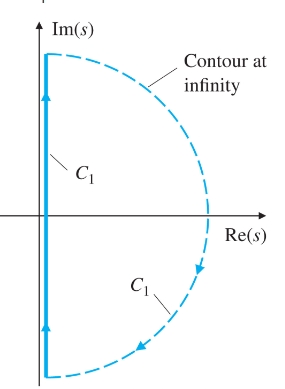
\includegraphics[width=.4\textwidth]{IMAGES/control/nyquist.png}
\end{figure}

Criteria : \begin{enumerate}
    \item Plot the Nyquist plot of $K(s)G(s)$\\
    \item Evaluate the number of clockwise encirclement of -1, call this N (+1 if clockwise, -1 if counter-clockwise)\\
    \item Determine the number of unstable poles of $G(s)$, call this P (in general $K(s)$ does not have unstable poles as we designed it)\\
    \item Calculate the number of unstable closed-loop roots Z : \begin{equation}
        Z = N+P
    \end{equation}
    \textbf{The closed-loop system is stable if and only if Z is zero.}\\
\end{enumerate}

\footnote{We do not consider the rest of the D-shape contour as $\lim_{\omega \rightarrow \infty} \lvert G(j\omega) \rvert = 0$. Plus the Nyquist plot is symmetric around the real axis.}

\quad \underline{Impact of integrator :}\\
Suppose the system is of the form : $K(s) G(s) = \frac{B(s)}{s^qA(s)}$. In order to compute the Nyquist, we follow a curve that takes an infinitesimal curve around the point $s=0$.\\

At $s_0=0$, we have : $K(s)G(s) = \frac{\gamma}{r^q}e^{-jq\theta}$, $\theta \in [-\frac{\pi}{2}, \frac{\pi}{2}]$.\\
\textbf{The nyquist plot will form a semi-circle with infinite radius oriented clockwise}.\\

\quad \underline{Simplified Nyquist criterion :}\\
\begin{theorem}
    If the open-loop system is stable and the -1 point lies to the left of the Nyquist curve, then the closed-loop system is stable.
\end{theorem}

\subsection{Robustness}
\subsubsection{Uncertain delay}
We designed for system $G(s)$ but in real word it might be : $G'(s) = G(s)e^{-s}$\\

The original system is stable but the delayed one might not be.\\

\subsubsection{Uncertain gain}
In real world, we might have $G'(s) = \alpha G(s)$\\
An uncertain gain generates some scaling. Even if the original system is stable, the one with larger gain might not be.\\

\quad \underline{Robustness :} The farther the nominal Nyquist curve is from the -1 point, the more likely the real system will be stable\\

\subsubsection{Gain margin}
The gain margin is the number $\frac{1}{a}$ where \begin{equation}
    a = \min_\omega K(j\omega) G(j\omega) \text{ such that } \Im K(j\omega) G(j\omega) = 0
\end{equation}

It is the amount that gain can increase while stable. Between $4dB$ and $12dB$ is considered safe. \\
$GM<1$ (0dB) means that the closed-loop system is unstable and $GM>1$ is stable.\\

On the Bode plot, it is the distance from 0 when the phase curve its -180$^\circ$.\\

\subsubsection{Phase margin}
The phase margin is the smallest increase in phase that will cause instability : \begin{equation}
    \phi = \min_{\phi, \omega} \phi \text{ such that } K(j\omega)G(j\omega) e^{j\phi} = -1
\end{equation}

Between $30^\circ$ and $60^\circ$ is considered safe.\\

On the Bode plot, it is the delta angle between -180$^\circ$ and the actual curve when the magnitude curve crosses 0.\\


\warning If there are multiple crossings, choose the first to be unstable.\\

\begin{figure}[hbt!]
    \centering
    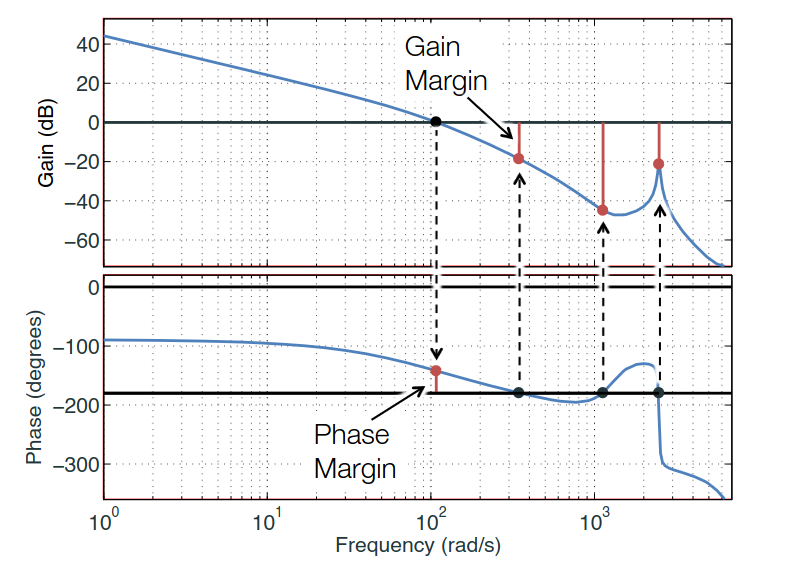
\includegraphics[width=.6\textwidth]{IMAGES/control/freq.png}
\end{figure}

\subsubsection{Delay margin}
Conversion of phase angle from angle to time : \\
Delay margin = $\frac{\text{Phase margin(rad) }}{\text{crossover frequency}}$\\





\subsection{Steady-state errors}
We have the following transfer function between the error and reference : $E(s) = \frac{R(s)}{1+K(s)G(s)} = S(s) R(s)$. Where $S(s)$ is called the \textbf{sensitivity function}.\\

Suppose that the open-loop transfer function has $q$ poles at $s=0$ : $K(s)G(s) = \frac{B(s)}{s^q A(s)}$ where $A$ and $B$ are polynomials.\\

\textbf{The number $q$ is called the type or class of the open-loop system.}\\

We define the open-loop steady-state gain of the system : $\gamma = \frac{B(0)}{A(0)}$\\

\quad \underline{Type 0 system :}\\

We apply a step input : $R(s) = \frac{1}{s}$\\

The steady-state error will be : \begin{equation}
    \lim_{t\rightarrow \infty} e(t) = \frac{1}{1+\gamma}
\end{equation}

\quad \underline{Type 1 system :}\\

We first apply a step input : $R(s) = \frac{1}{s}$\\
The steady-state error will be zero for all step inputs and systems.\\

We apply a ramp input : $r(t) = t$\\

The steady-state error is : $\lim_{t\rightarrow \infty} e(t) = \frac{1}{\gamma}$\\
Non-zero steady-state error.\\

We now apply a parabolic input $r(t) = t^2$\\
$E(s) = \frac{B(s)}{sA(s)+B(s)} \frac{2}{s^2}$\\
We cannot apply the final-value theorem because there is more than one pole at 0. The error is either unbounded or oscillates.\\

\quad \underline{Generalisation :}\\
Let $R = \frac{1}{s^{r+1}}$ and $KG = \frac{B}{A} \frac{1}{s^q}$\\
Then $\lim_{t\rightarrow \infty} e(t) = \lim_{s\rightarrow 0} \frac{s^{q-r}}{s^q+\frac{B}{A}} = \begin{cases}
    q<r \rightarrow \infty\\
    q=r \rightarrow \frac{1}{\gamma}\\
    q>r \rightarrow 0\\
\end{cases}$

\begin{table}[hbt!]
    \centering
    \begin{tabular}{c c c c}
        Type & $r(t) = 1$ & $r(t) = t$ & $r(t) = t^2$ \\ \hline
        0 & $\frac{1}{1+\gamma}$ & $\infty$ & $\infty$\\ \hline
        1 & 0 & $\frac{1}{\gamma}$ & $\infty$\\ \hline
        2 & 0 & 0 & $\frac{1}{\gamma}$\\
    \end{tabular}
\end{table}

Although, the presence of integrator reduce the gain and phase margin. The more integrator, the less stable the system will become.\\

\subsection{Constant disturbance rejection}
The system response with respect to a disturbance $w(t)$ is : $E(s) = \frac{G(s)}{1+K(s)G(s)} W(s)$\\

If the system has $q$ integrator and K has none, the error will be : $E(s) = \frac{B(s)}{s^q A(s) + K(s) B(s)} \frac{1}{s}$\\
Then the steady-state error is : $\lim_{s\rightarrow 0} sE(s) = \frac{1}{K(0)}$\\
Integrator in the system do not reject disturbances!\\


Now, if K has $r$ integrator, the error is : $E(s) = s^{r-p} \frac{B(s)R(s)}{s^{q+r}A(s) R(s) + S(s)B(s)}$ (p the order of $R(s)$ i.e. p=1 for a step input)\\
In order to reject the disturbance, we need the number of integrator in the system plus the number of integrator in the controller to be greater then the complexity of the system.\\

\subsection{Waterbed effect}
We want to reject complex signals. Consider a sinusoid or a mix of them. The rejection of these signals is given by the sensitivity function : $\lvert S(j\omega)\rvert = \lvert \frac{1}{1+K(j\omega) G(j\omega)}\rvert$\\

\begin{theorem}
    Assume we have a closed-loop stable system with open-loop unstable poles $p_i$ (i=1,$\dots$,P) and a strictly proper open-loop transfer function $K(s)G(s)$. The sensitivity function satisfies the condition : \begin{equation}
        \int_0^\infty \log \lvert S(j\omega)\rvert d\omega = \pi \sum_{i=1}^P \Re(p_i)
    \end{equation}
\end{theorem}

\begin{itemize}
    \item If we damp noise for some frequencies ($\lvert S(j\omega) \rvert < 1$), then we must amplify it at some others\\
    \item Harder to get good disturbance rejection behaviour out of unstable systems.\\
\end{itemize}

\subsection{Loop shaping}
Closed-loop transfer function are a highly nonlinear function of the control law. Although, the response KG is linear in K and therefore much easier.\\

\subsubsection{Sensitivity and complementary sensitivity}
\begin{itemize}
    \item Response of error E(s) to output noise V(s) : \textbf{sensitivity function} \begin{equation}
        S(s) = \frac{1}{1+G(s)K(s)}
    \end{equation}
    It corresponds to the impact of noise on the error. \textbf{Ideal value : 0}\\
    \item Response of output Y(s) to reference R(s) : \textbf{complementary sensitivity function} \begin{equation}
        T(s) = \frac{K(s)G(s)}{1+K(s)G(s)}
    \end{equation}
    It corresponds to the impact of reference on the output. \textbf{Ideal value : 1}\\
\end{itemize}

These functions are complementary : $T(s)+S(s) = 1$; changes in one will cause changes in the other.\\
We mostly want good tracking and noise rejection at low frequencies and bad at high.\\

\begin{figure}[hbt!]
    \centering
    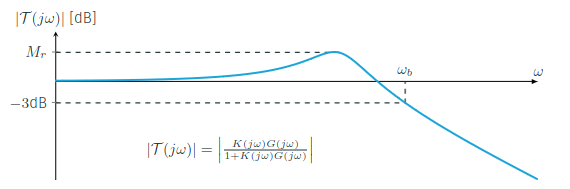
\includegraphics[width=.8\textwidth]{IMAGES/control/sensitivity.png}
\end{figure}

The desired shape is : \begin{itemize}
    \item Low-frequency gain of 0dB\\
    \item Small resonance peak $M_r$\\
    \item Large bandwidth defined by the pass-band [0,$\omega_b$] and the cutoff-frequency $\omega_b$\\
    \item Hgh roll-off after $\omega_b$ to make the system insensitive to measurement noise\\
\end{itemize}

Both functions should look like : \begin{figure}[hbt!]
    \centering
    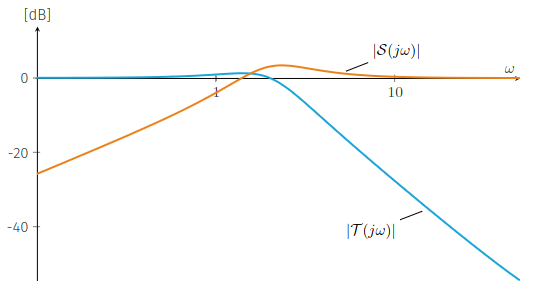
\includegraphics[width=.5\textwidth]{IMAGES/control/sensitivity2.png}
\end{figure}

\warning After the cutoff-frequency, we cannot trust sensors and the controller should be turned off.\\
Higher the gain, greater the bandwidth but less robust the system becomes.\\

We have : $T(j\omega) = 1-\frac{1}{1+K(j\omega)G(j\omega)}$ \begin{itemize}
    \item $T(j\omega) = 1$ for small $\omega$ $\Leftrightarrow K(j\omega)G(j\omega)$ large\\
    \item $\lvert T(j\omega)\rvert <<0dB$ for large $\omega$ $\Leftrightarrow \lvert K(j\omega)G(j\omega) \rvert<<0dB$\\
    \item Low resonance peak, or large stability margins\\
    \item Open-loop crossover frequency (0dB) $\simeq$ Closed-loop bandwidth\\
\end{itemize}

Let define \textbf{Loop gain} : $L(s) = K(s)G(s)$. Low-frequency slope and gain are chosen for steady-state error.\\
The open-loop frequency response has been designed for : \begin{itemize}
    \item $\lvert KG(j\omega)\rvert >>1$ for $\omega<<\omega_c$\\
    \item $\lvert KG(j\omega)\rvert <<1$ for $\omega >> \omega_c$\\
\end{itemize}

The closed-loop response is therefore : \begin{equation}
    \lvert T(j\omega)\rvert = \begin{cases}
        1 & \omega << \omega_c\\
        \lvert KG\rvert & \omega>> \omega_c\\
    \end{cases}
\end{equation}

Around crossover, $\lvert KG(j\omega)\rvert \simeq 1$, if $\phi$ is the phase margin, we have : \begin{equation}
    \lvert T(j\omega)\rvert = \lvert \frac{-e^{-j\phi}}{1-e^{-j\phi}}\rvert
\end{equation}

The closed-loop bandwidth is within a factor of two of the crossover frequency but as we use log axis we can approximate it to the crossover frequency : $\omega_c \leq \omega_{BW} \leq 2\omega_c$\\

Let's take for example : $G(s) = \frac{\omega_n^2}{s(s+2\xi \omega_n)}$\\
$T(s) = \frac{\omega_n^2}{s^2+2\xi \omega_n s+\omega_n^2}$ (unit feedback)\\

The phase margin can be approximated by : $PM \simeq 100\xi$\\

Then, we have the following graph : \begin{figure}[hbt!]
    \centering
    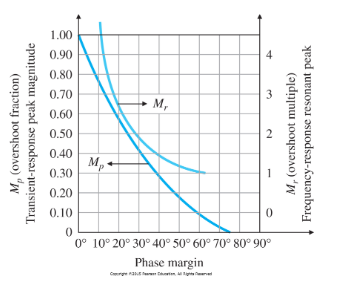
\includegraphics[width=.5\textwidth]{IMAGES/control/mpmr.png}
\end{figure}

The damping ratio determines the step response overshoot and the size of the resonant peak.\\

We now need to choose K(s) that satisfies desired requirements. In order to do that, we can use different tools : overall gain, lead compensator and lag compensator.\\

\subsubsection{Lead compensator}
\begin{equation}
    D_c(s) = \frac{T_Ds+1}{\alpha T_Ds+1}
\end{equation}
With $\alpha<1$\\
It helps to increase phase margin. Within interval of interest, the phase increases by $\phi_{max}$ and the slope increases by 20dB/dec.\\

\begin{figure}[hbt!]
    \centering
    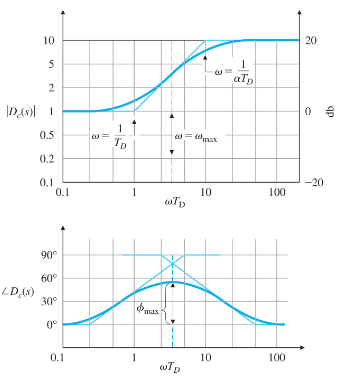
\includegraphics[width=.5\textwidth]{IMAGES/control/leadcomp.png}
\end{figure}

Max phase increase happens at the center of the pole and zero. The amount of phase lead at this point is : \begin{equation}
    \begin{gathered}
        \omega_{max} = \frac{1}{T_D \sqrt{\alpha}}\\
        \sin \phi_{max} = \frac{1-\alpha}{1+\alpha} \Rightarrow \alpha = \frac{1-\sin \phi}{1+\sin \phi}\\
    \end{gathered}
\end{equation}

\quad \underline{Design procedure :}\\
\begin{itemize}
    \item Choose system type and controller gain K\\
    \item Determine the increase in phase margin required (add about 10-15$^\circ$ to compensate for bandwidth increase) and choose $\alpha$\\
    \item Choose $\omega_{max}$ to be the crossover frequency\\
\end{itemize}

A low slope at crossover provides a good phase margin (-20dB/dec gives a phase margin of 90$^\circ$). The slope must be constant for a decade around the crossover frequency for the approximation to hold.\\

\subsubsection{Gain-phase relationship}
\begin{theorem}
    For any stable minimum-phase system the phase of $G(j\omega)$ is uniquely related to the magnitude of $G(j\omega)$ : \begin{equation}
       \langle G(j\omega_0) = \frac{1}{\pi} \int_{-\infty}^\infty (\frac{dM}{du})W(u)du 
    \end{equation} 
    In radians, where $M = \ln\lvert G(j\omega)\rvert$, $u=\ln \frac{\omega}{\omega_0}$, $W(u) = \ln \frac{\coth\lvert u \rvert}{2}$\\
\end{theorem}

Simple form : $\langle G(j\omega) \simeq n 90^\circ$ where n is the slope of $\lvert G(j\omega)\rvert$ in units of decade of amplitude per decade of frequency.\\

We define a decade as 10. Therefore, if we want to find the frequency half a decade before $\omega_0$ it is located at $\frac{\omega_0}{3}$ and half a decade after $3\omega_0$.\\

If $\alpha\rightarrow 0$, then $K(s) = K(1+T_Ds)$ a PD controller.\\

\subsubsection{Lag compensator}
\begin{equation}
    D_c(s) = \frac{T_Is+1}{\alpha T_Is+1}
\end{equation}

Within the interval of interest : \begin{itemize}
    \item phase decreased by up to $90^\circ$\\
    \item Gain increased below $\frac{1}{T_I}$
\end{itemize}

The goal is to increase the gain at low frequencies to reduce steady-state errors. The phase goes back to 0 after $\frac{1}{T_I}$\\
In order to not disturb the phase at crossover frequency, we usually take $\frac{1}{T_I} = \frac{\omega_c}{5}$.\\

If $\alpha \rightarrow \infty$, $KD_c(s) = K(1+\frac{1}{T_Is})$, then we have a PI controller.\\

Choose point where phase is the one we want. Record the gain at this point. We want to move the gain bode plot upwards such that the new crossover frequency is this point. Find alpha as : $\frac{1}{\alpha} = -GM$ at this point and in dB that we need to convert in decimal \warning \\

\subsubsection{Lead/Lag compensator}
\begin{itemize}
    \item lead compensator : \textbf{adds phase} at crossover frequency to improve margins. Impacts frequencies above the breakpoint\\
    \item lag compensator : \textbf{adds gain} at low frequency to improve the steady-state response. Impacts frequencies below the breakpoint\\
\end{itemize}

The lead compensator can be a PD controller whereas the lag compensator can be a PI controller.\\

\begin{equation}
    D_c(s) = K(T_Ds+1)(1+\frac{1}{T_Is})
\end{equation}

\subsubsection{Notch filter}
If the phase that we have to gain is too important, than we might want to use a Notch filter. It is a lead compensator for poles of degree 2.\\
\begin{equation}
    N = \frac{(\frac{s}{\omega_n})^2 + 2 \frac{\xi_n}{\omega_n}s+1}{((\frac{s}{\omega_p})^2 + 2 \frac{\xi_p}{\omega_p}s+1) (\frac{s}{p}+1)}
\end{equation}
We try to put the notch before the resonant frequency.\\


\subsection{State-space}
This is equivalent to the transfer function form studied previously : $\begin{matrix}
    \dot{x} = Ax+Bu\\
    y = Cx + Du\\
\end{matrix}$\\

Procedure : \begin{enumerate}
    \item State-feedback design : assume that the state is measured and design a static control law $u=Kx$\\
    \item State observer : design a dynamic system to estimate the state : $\dot{\hat{x}} = L\hat{x} + My + Nu$, design $L,M,N$ such that $\hat{x} \simeq x$\\
\end{enumerate}

\subsubsection{Dynamic response}
Take Laplace transform of the state-space : \begin{equation}
    \begin{gathered}
        X(s) = (sI-A)^{-1}BU(s) + (sI-A)^{-1}x(0)\\
        Y(s) = (C(sI-A)^{-1}B+D)U(s) + C(sI-A)^{-1}x(0)\\
        G(s) = C(sI-A)^{-1}B+D\\
    \end{gathered}
\end{equation}

\subsubsection{Poles}
Poles are complex frequencies the system will respond at without a forcing function.\\

Consider $\dot{x} = Ax$, if p is a pole of the system then $x(t) = e^{pt}x_0$\\
\warning Therefore, poles are eigenvalues of A\\

\textbf{Poles are the solutions of the characteristic equation} \begin{equation}
    det(sI-A)=0
\end{equation}

\subsubsection{Zeros}
Zeros are generalized frequencies at which the system will not respond to an input : $y(t) = 0$\\

After solving, we get that zeros are points where : \begin{equation}
    det \begin{pmatrix}
        zI-A & -B\\
        C & D\\
    \end{pmatrix} = 0
\end{equation}

\subsubsection{Canonical forms}
Two state representations can have exactly the same input-output behaviour.\\
The control canonical form allows for simple modification of the system dynamics.\\
Consider the transfer function, we get the control canonical form : \begin{equation}
    \begin{gathered}
        G(s) = \frac{b_1s^{n-1} + \dots + b_{n-1}s + b_n}{s^n + a_1 s^{n-1} + \dots + a_{n-1}s+a_n}\\
        A = \begin{pmatrix}
            -a_1 & -a_2 & \dots & \dots & -a_n\\
            1 & 0 & \dots & \dots & 0\\
            0 & 1 & 0 & \dots & 0\\
            \vdots & \vdots & \vdots & 0 & \vdots\\
            0 & 0 & \dots & 1 & 0\\
        \end{pmatrix}\\
        B = \begin{pmatrix}
            1\\ 0 \\ \vdots \\ 0\\
        \end{pmatrix}\\
        C = \begin{pmatrix}
            b_1 & b_2 & \dots & b_n\\
        \end{pmatrix}\\
        D = 0\\
    \end{gathered}
\end{equation}

\warning If $b_0$ is non zero, this is not valid!\\

The state equations are not unique. We can have a change of variables : $x=Tz$. Therefore : \begin{itemize}
    \item $\dot{z} = T^{-1}ATz + T^{-1}Bu = \overline{A} z + \overline{B}u$\\
    \item $y = CTz + Du = \overline{C} z  + \overline{D}u$\\
\end{itemize}

It is the same dynamic system.\\

General procedure for state transformation to control canonical form : \begin{itemize}
    \item From the controllability matrix : $C = \begin{pmatrix}
        B & AB & A^2B & \dots & A^{n-1}B\\
    \end{pmatrix}$\\
    \item Compute the last row of the inverse : $t_n = \begin{pmatrix}
        0 & 0 & \dots & 1\\
    \end{pmatrix}C^{-1}$\\
    \item Construct the transformation matrix : $T^{-1} = \begin{pmatrix}
        t_n A^{n-1}\\ t_n A^{n-2}\\ \vdots \\ t_n\\
    \end{pmatrix}$
\end{itemize}

\warning The system can only be put in controllable form if $C$ is full rank.\\

\subsubsection{Full state feedback}

First, we can try a static linear control law : $u = -Kx$\\
By doing so, we can place n poles.\\
Closed loop dynamics are : $\dot{x} = (A-BK)x$\\

Poles are given by the characteristic equation \begin{equation}
    det(sI-(A-BK)) = (s-s_1)\dots (s-s_n)
\end{equation}

In control canonical form, we have : $A-BK = \begin{pmatrix}
    -a_1 - K_1 & \dots & -a_n-K_n\\
    1 & \dots & 0\\
    \vdots & \vdots & \vdots\\
    0 & \dots & 0\\
\end{pmatrix}$\\

Characteristic equation is : $c(s,K) = s^n + (a_1 + K_1)s^{n-1} + \dots + (a_n + K_n)$\\
And the target is : $\alpha_c(s) = s^n + \alpha_1 x^{n-1} + \dots + \alpha_n$\\

Control law is : \begin{equation}
    K = [-a_1 + \alpha_1 \quad \dots \quad -a_n + \alpha_n]
\end{equation}

\quad \underline{Pole placement in Control Canonical Form :}\\
Two possibilities : \begin{enumerate}
    \item Procedure to place poles at desired locations $s_i$ given dynamic system (A,B) : \begin{itemize}
        \item Compute transformation matrix T to conver to to control canonical form ($A_c$, $B_c$)\\
        \item Compute control law $K_c$ to place poles\\
        \item Convert control gain back to original state $K = K_c T^{-1}$\\
    \end{itemize}
    \item \textbf{Ackermann's formula} : (all in one computation), choose controller gain K for the system (A,B) so that the closed-loop system $\dot{x} = (A-BK)x$ has the characteristic equation $\alpha(s)$ \begin{equation}
        \begin{gathered}
            K = [0\quad 0 \quad \dots \quad 1] \mathcal{C}^{-1} \alpha(A)\\
            \text{where } \alpha(A) = A^n + \alpha_1 A^{n-1} + \dots + \alpha_n I\\
        \end{gathered}
    \end{equation}
\end{enumerate}

A static linear controller $u=-Kx$ can place the closed-loop poles arbitrarily. Controllability matrix $\mathcal{C}$ must be invertible.\\

\subsubsection{Controllability}
An LTI system is controllable if, for every $x^*$ and every T>0, there exists an input function $u(t)$, $0<t\leq T$ such that the state goes from $x(0)=0$ to $x(T)=x^*$.\\

\begin{theorem}
    The LTI system $(A,B)$ is controllable if and only if rank($\mathcal{C}$) = n where $A\in \mathbb{R}^{nxn}$\\
\end{theorem}

\textbf{State transformation do not impact controllability}.\\

\subsubsection{Modal canonical form}
Assume transfer function has distinct real poles $p_i^2$.\\
\begin{equation}
    G(s) = \frac{N(s)}{(s-p_1)\dots(s-p_n)} = \frac{r_1}{s-p_1} + \dots + \frac{r_n}{s-p_n}
\end{equation}

We can define a set of first-order systems, each with their own state.\\
Then we can write the modal canonical form with A diagonal : \begin{equation}
    \begin{gathered}
        \dot{x} = \begin{pmatrix}
            p_1 & &\\
             & \dots & \\
              & & p_n\\
        \end{pmatrix}x + \begin{pmatrix}
            1\\ \vdots \\ 1\\
        \end{pmatrix}u\\
        y = [r_1 \dots r_n]x\\
    \end{gathered}
\end{equation}

In order to do so, we decompose $A = T\Lambda T^{-1}$, with $\Lambda$ the eigenvalues of A and T the eigenvectors. We then apply the state transformation $x = Tz$\\
And we get : $\dot{z} = \Lambda z + T^{-1} Bu$, $y = CTz + Du$\\

\subsubsection{Reference tracking}
If the state input pair $(x_{ss}, u_{ss})$ satisfies the conditions : \begin{equation}
    \begin{gathered}
        0 = Ax_{ss} + Bu_{ss}\\
        r = C x_{ss} + Du_{ss}\\
    \end{gathered}
\end{equation}
And the control law $u = u_{ss} -K(x-x_{ss})$ is applied, then $\lim_{t\rightarrow \infty}y(t) = r$\\

We therefore have : \begin{equation}
    \begin{pmatrix}
        x_{ss}\\ u_{ss}\\
    \end{pmatrix} = \begin{pmatrix}
        A & B\\ C & D\\
    \end{pmatrix}^{-1} \begin{pmatrix}
        0 \\1\\
    \end{pmatrix}r = \begin{pmatrix}
        N_x\\N_u\\
    \end{pmatrix}r
\end{equation}

The controller is now : $u = -Kx + (N_u + KN_x)r = -Kx + \overline{N}r$\\

\subsubsection{Selection of good pole approximation}

There are many ways to do such things : \begin{enumerate}
    \item Place dominant second-order poles : choose location for the main behaviour wanted and damped the rest of the modes quickly (put them about 4 or 5 times further away)\\
    \item Model matching : choose from a parameterized prototype response.\\
    \item Optimal control : Linear Quadratic Regulator\\
\end{enumerate}

\quad \underline{Dominant pole approximation :}\\
Choose the closed-loop system to have an almost second-order response.\\

\quad \underline{Model matching :}\\
Select characteristic equation that is known to give good response.\\

I.E. Bessel polynomials : \begin{equation}
\begin{gathered}
    \theta_n(s) = \sum_{k=0}^n a_k s^k\\
    a_k = \frac{(2n-k)!}{2^{n-k}k! (n-k)!}\\
    \end{gathered}
\end{equation}

\warning Settling time is always 1 : need to scale it $\frac{P}{T_s}$\\

\subsection{State observers}

The goal is to estimate the state from input and output measurements. If $\hat{x}$ is our estimate of the state and we simulate the dynamics $\dot{\hat{x}} = A\hat{x} + Bu$\\
Noise and model error will cause the estimate to diverge so we add \textbf{feedback} : \begin{equation}
    \dot{\hat{x}} = A\hat{x} + Bu + L(y-C\hat{x})
\end{equation}

Dynamics representing the error is : $\dot{e} = \dot{x}-\dot{\hat{x}} = (A-LC)e$\\
We need to choose L such that the error system is stable. \\

The observer canonical form is written as : \begin{equation}
    \begin{gathered}
        \dot{x} = \begin{pmatrix}
            -a_1 & 1 & 0\\
            -a_2 & 0 & 1\\
            -a_3 & 0 & 0\\
        \end{pmatrix} x  + \begin{pmatrix}
            b_1\\ b_2 \\b_3\\
        \end{pmatrix}u\\
        y = [1 \quad 0 \quad 0]x\\
    \end{gathered}
\end{equation}

In order to transform it to observer canonical form, we can use the formula of the determinant such that : \begin{equation}
    det(sI-(A-LC)) = s^n + (a_1+L_1)s^{n-1} + \dots + (a_n+L_n)
\end{equation}

In general, we have the following : \begin{equation}
    \begin{gathered}
    G(s) = \frac{b_1 s^{n-1} + \dots + b_n}{s^n + a_1 s^{n-1} + \dots + a_n}\\
        A = \begin{pmatrix}
            -a_1 & 1 & 0&0\\
            -a_2 & 0 & 1&0\\
            \vdots & \vdots&\vdots & \vdots\\
            -a_n & 0&0 & 0\\
        \end{pmatrix}\\
        B = \begin{pmatrix}
            b_1\\ \vdots \\ b_n\\
        \end{pmatrix}\\
        C = \begin{pmatrix}
            1 & 0 & \dots & 0\\
        \end{pmatrix}\\
    \end{gathered}
\end{equation}

For the error dynamics to always be 0, we need $det(sI-A+LC) = 0$\\
Observer poles can be placed easily if system can be put in observer canonical form.\\
The transfer function can be written as : \begin{equation}
    G(s) = C (sI-A+LC)^{-1}L
\end{equation}
\warning C can be different from before depending and the transfer function we want\\

For pole placement, we can use \textbf{Ackermann's estimator formula} : \\
Choose observer gain L for the system (A,C) so that the closed-loop system $\dot{e} = (A-LC)e$ has the characteristic equation $\alpha_e(s)$ \begin{equation}
    L = \alpha_e(A) \mathcal{O}^{-1} \begin{pmatrix}
        0\\0\\ \dots \\ 1\\
    \end{pmatrix}
\end{equation}
where $\alpha_e(A)$ is the desired characteristic equation : $\alpha_e(A) = A^n + \beta_1 A^{n-1} + \dots + \beta_n$\\

With $\mathcal{O}$ the observability matrix : \begin{equation}
    \mathcal{O} = \begin{pmatrix}
        C \\ CA\\ \vdots \\ CA^{n-1}\\
    \end{pmatrix}
\end{equation}

\textbf{LTI system (A,C) is observable if and only if the observability matrix is full rank} : rank($\mathcal{O}$)=n\\

\footnote{Observer pole placement is identical to controller pole placement if we replace (A,B) with $(A^T, B^T)$}

\quad \underline{Pole selection :}\\
Estimator pole selection is a trade-off between sensor noise and transient response. : \textbf{Estimator poles should be faster than the controller poles by about 2-6 times.}\\
\begin{itemize}
    \item Faster estimator : more sensor noise passed to controller\\
    \item Slower estimator : slower transient response\\
\end{itemize}

\subsubsection{Combining control and estimation}

Full-state feedback controller : $\dot{x} = Ax-BK\hat{x}$\\
Observer : $\dot{\hat{x}} = A\hat{x} - BK\hat{x} + L(y-C\hat{x})$, $\dot{e} = (A-LC)e$\\

\begin{equation}
    \begin{pmatrix}
        \dot{x}\\ \dot{e}\\
    \end{pmatrix} = \begin{pmatrix}
        A-BK & BK\\
        0 & A-LC\\
    \end{pmatrix}
\end{equation}
Compared to a feedback controller, we have $A=A^T$ and $B=C^T$\\
And the transfer function will look like : \begin{equation}
    K(s) = -K(sI-A+LC+BK)^{-1}L
\end{equation}

By \textbf{separation principle} : the poles of the closed-loop system are $det(sI-A+BK)det(sI-A+LC) = \alpha_c(s) \alpha_e(s) = 0$\\

\subsubsection{Reference input}
We now add a reference as a linear input to the controller : \begin{equation}
    \begin{gathered}
        \dot{\hat{x}} = (A-BK-LC)\hat{x} + Ly + Mr\\
        u = -K\hat{x} + \overline{N}r\\
    \end{gathered}
\end{equation}

How do we choose M and N?\\
\warning The reference cannot impact the pole locations. It does change the zeros.\\

Two options : \begin{itemize}
    \item Autonomous Estimator : Estimator is estimating the state of the system and so should not be impacted by the reference. \textbf{Select M and $\overline{N}$ so that the state estimator is independant of r} \begin{equation}
        B\overline{N} = M
    \end{equation}
    The estimated state $\hat{x}$ does not have the reference as an input. \textbf{Selection of $\overline{N}$ is the same as in the full state-feedback.} (ensure zero tracking error in steady-state\\
    \item Tracking-error estimator : use only $e=r-y$ in the estimator. Used when only the error is measured. Choose M and $\overline{N}$ such that the estimator only uses $e=r-y$ \begin{equation}\begin{gathered}
        \overline{N} = 0\\
        M = -L\\
        \text{controller is now : } \dot{\hat{x}} = (A-BK-LC)\hat{x} + L(y-r) = (A-LC)\hat{x} + LCx +Bu\\
        u=-K\hat{x}\\
        \end{gathered}
    \end{equation}
\end{itemize}

\subsubsection{Integral control}
As we do not have any integrator in the control loop, steady-state offset is likely. \\
We define an artificial state that is the integral of the error : $x_I(t) = \int_0^t e(\tau)d\tau$ where $\dot{x_I}(t) = e(t)$\\

The augmented system model is : \begin{equation}\begin{gathered}
    \begin{pmatrix}
        \dot{x}\\ \dot{x}_I\\
    \end{pmatrix} = \begin{pmatrix}
        A & 0\\ -C & 0\\
    \end{pmatrix} \begin{pmatrix}
        x \\ x_I\\
    \end{pmatrix} + \begin{pmatrix}
        B\\0\\
    \end{pmatrix}u + \begin{pmatrix}
        0\\1\\
    \end{pmatrix}r\\
    y = [C \quad 0 ] \begin{pmatrix}
        x\\ x_I\\
    \end{pmatrix}
    \end{gathered}
\end{equation}

Again, the controller will have the form : \begin{equation}
    u = -[K_0 \quad K_1] \begin{pmatrix}
        x\\ x_I\\
    \end{pmatrix}
\end{equation}

\subsection{Linear Quadratic Regulator}
The goal is to move from state $x$ to the origin.\\
We have the cost of being in state $x$ as : $l(x,u) = x^TQx + u^TRu$.\\

The total cost of following a particular trajectory is : \begin{equation}
    V(x,u) = \int_0^\infty x(t)^TQx(t) + u(t)^TRu(t)dt
\end{equation}

Assume R positive definite and Q positive semi-definite.\\

The best trajectory is : $\min_u V(x(t),u(t))$.\\

Usually, we start with $Q = C^TC$ and $R=  \rho I$\\
Therefore, $V(x,u) = \int_0^\infty y(t)^2 + \rho u(t)^2dt$ which is the energy in the input and output signals.\\

\quad \underline{Optimal solution :}\\
The optimal controller is $u(t) = -Kx(t) = u_0$ where \begin{equation}
    K = R^{-1} B^TP
\end{equation}
And $P = P^T$ is the solution of the Riccati Equation : \begin{equation}
    A^TP + PA-PBR^{-1}B^TP + Q = 0
\end{equation}

A quantity is called \textbf{feedback invariant} if its value does not depend on the choice of the control input $u(t)$, $t\geq 0$\\
\begin{theorem}
    Let P be a symmetric matrix. For every control input $u(t)$, $t\in [0,\infty]$ for which $x(t)\rightarrow 0$ as $t\rightarrow \infty$, we have that \begin{equation}
        \int_0^\infty x^T(A^TP+PA)x+2x^TPBudt = -x(0)^TPx(0)
    \end{equation}
\end{theorem}

\subsubsection{Choice of weights}
Weights are usually determined through a trial and error process but we can start with Bryson's rule : \\
Choose diagonal Q and R with :
\begin{itemize}
    \item $Q_{ii} = \frac{1}{\text{maximum acceptable value of }x_i^2}$\\
    \item $R_{jj} = \frac{1}{\text{maximum acceptable value of }u_j^2}$\\
\end{itemize}

\subsection{Discrete-time implementation}
Sensors are discrete-time : they can only see the world at fixed time intervals.\\

We normally sample with a constant sampling period $T = t_k - t_{k-1} \forall k\in \mathbb{Z}$\\
Sampling frequency : $f = \frac{1}{T}$Hz and $\omega = 2\pi f$ rad/sec\\

The nyquist theorem tells us that we need to sample at least twice as fast as the highest frequency of the system (usually about 20-40).\\

A linear difference equation of order n : \begin{equation}
    y(k) + a_1y(k-1)+ \dots + a_ny(k-n) = b_0 u(k-d) + b_1 u(k-d-1) + \dots + b_m u(k-d-m)
\end{equation}

\begin{itemize}
    \item d is the system delay\\
    \item can compute the value of $y$ at time $k$ given last n outputs (y) and m inputs from d steps ago (u(k-d))\\
\end{itemize}

\textbf{Shift operator :} \begin{equation}
    \begin{gathered}
        zy(k) = y(k+1)\\
        z^{-1}y(k) = y(k-1)\\
    \end{gathered}
\end{equation}

Therefore, the discrete time transfer function is : \begin{equation}
    \frac{Y(z)}{U(z)} = H(z) = \frac{z^{-d}(b_0 + b_1z^{-1}+ \dots + b_m z^{-m})}{1+ a_1z^{-1} + \dots + a_n z^{-n}}
\end{equation}

We now need to approximate the transfer function in discrete time. For that, we use : \begin{equation}
s \simeq \frac{2}{T} \frac{z-1}{z+1}\end{equation}









\end{document}